\documentclass[aspectratio=169,usenames,dvipsnames]{beamer}
\usepackage[T1]{fontenc}
\usepackage{graphicx}
\usepackage{multicol}
\usepackage{ulem}
\graphicspath{ {./images/} }

\usetheme{mittens}

% Possible color schemes: \colorschemered, \colorschemeblue, \colorschemegreen, \colorschemebrown, \colorschemepurple
\colorschemered

% Comment this line out to disable section & subsection names at the top of slides
\sectionnamestrue

% Comment this line out to remove new section slides
\sectionslidestrue

\title{Partial Solution of 3 x N Chomp boards in the form of [2, H, 2]}
\author[E. Skwarka]{Ezra Skwarka}
\date[2021]{October 2021}

\begin{document}
\titleslide

% Summer Research Project
\begin{frame}{fragile}
    \frametitle{Summer Research Project}

    \begin{itemize}
        \item Summer Research 2020
        \item With Dr. B
        \item Combinatorial Games, specifically Chomp
    \end{itemize}
\end{frame} 

% Overview
\begin{frame}{fragile}
    \frametitle{Summer Research Project}

    \begin{enumerate}
        \item What is the Combinatorial Game Chomp?
        \item So What Did I Do?
        \item Divide and Conquer
        \item Postamble
    \end{enumerate}
\end{frame} 


%%%%%%%%%%%%%%%%%%%%%%%%%
\section{What is the Combinatorial Game Chomp?}

% What Makes a Combinatorial Game?
\begin{frame}{fragile}
    \frametitle{What Makes a Combinatorial Game?}

    \begin{itemize}
        \item Deterministic, no randomness
        \item Perfect Information, nothing is hidden
    \end{itemize}
    \text{$  $}
    \begin{itemize}
        \item Two types:
            \begin{itemize}
            \item Finite, the game will end, you can't loop
            \item Infinite, the game may not end, you can create loops
            \end{itemize}
    \end{itemize}
\end{frame} 

% But what is Chomp?
\begin{frame}{fragile}
    \frametitle{But what is Chomp?}

    \begin{itemize}
        \item Played on a board like a chocolate bar where the lower left piece is poisoned
        \item You don’t want to eat the poison, unless you’ve built up a resistance to iocane powder
        \item Alternating turns where you choose a piece and break off all pieces above and to the right of it
    \end{itemize}
\end{frame}

% What Are The Different Board Types?
\begin{frame}{fragile}
    \frametitle{What Are The Different Board Types?}

    \begin{itemize}
        \item Prescriptive: 2 x N, N x N
        \item Pictographic: just a picture\\ 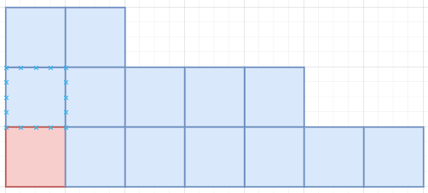
\includegraphics[scale=0.75]{[2, 3, 2].png}
        \item Long form: truncated, lists columns by height 
        \begin{itemize}
            \item $\texttt{\{}3, 3, 2, 2, 2, 1, 1\texttt{\}}$
        \end{itemize}
        \item Short Form: truncated, lists width of groups of column heights 
        \begin{itemize}
            \item $[2, 3, 2]$
        \end{itemize}
    \end{itemize}
\end{frame}

% What Has Already Been Done?
\begin{frame}{fragile}
    \frametitle{What Has Already Been Done?}

    \begin{itemize}
        \item $1$ x $N$: Go first, leave only poisoned piece\\
        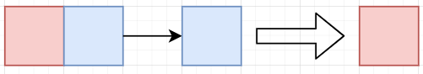
\includegraphics[scale=.5]{1 x N key.png}
        \item $N$ x $N$: Go first, make an L, Tweedledee-Tweedledum\\
        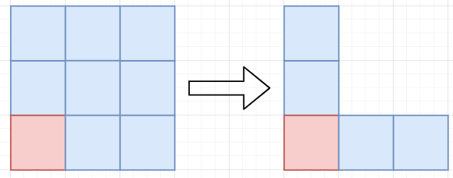
\includegraphics[scale=.5]{N x N key.png}
        \item $2$ x $N$: Go first, take top right, Tweedledee-Tweedledum\\
        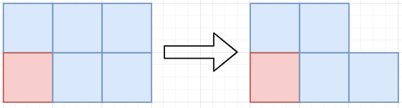
\includegraphics[scale=.5]{2 x N key.png}
    \end{itemize}
\end{frame}

% How Do I Know If I'm Winning?
\begin{frame}{fragile}
    \frametitle{How Do I Know If I'm Winning?}

    \begin{itemize}
       \item Winning and losing positions (P vs N)
        \begin{itemize}
            \item Every board has a recursively defined Nim Number, but they blew up too fast
        \end{itemize} 
        \item Looking at 3 x N boards\\
        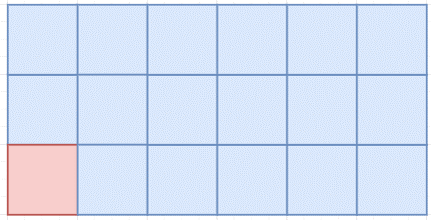
\includegraphics[scale=.5]{3 x 6 board.png}
        \begin{itemize}
            \item Note the arrow can be any number of blocks including zero
            \item I call this an “H-block”\\
            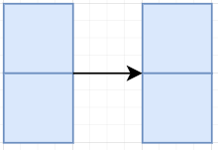
\includegraphics[scale=.25]{2 H block.png}
        \end{itemize}
    \end{itemize}
\end{frame}

%%%%%%%%%%%%%%%%%%%%%%%%%%%%%%%%%%%%%%%%%%%%%%%%%%%

%%%%%%%%%%%%%%%%%%%%%%%%
\section{So What Did I Do?}

% Data Mining with the Short Form
\begin{frame}{fragile}
    \frametitle{Data Mining with the Short Form}
    
    \begin{itemize}
        \item Wrote a Python script to iterate through all boards from a maximum size to get its position state and those of its children recursively with memoization.
        \begin{itemize}
            \item Work toward the base case, can exit early
            \item Code on my GitHub for the curious
        \end{itemize}
        \item Noticed a pattern in the Long Form, but it was hard to see, so I made the Short Form
        \begin{itemize}
            \item $\texttt{\{}3, 3, 2, … 2, 1, 1\texttt{\}}$ was always a winning position
            \item $[2, H, 2]$
        \end{itemize}
        \item Saw a pattern, tried to prove it
    \end{itemize}
\end{frame}

% Building a Seeded Kindergarten
\begin{frame}{fragile}
    \frametitle{Building a Seeded Kindergarten}
    \text{Two ways to generate the children:}
    \begin{itemize}
        \item Generating the first generation of children visually
        \item Generating the first generation of children algorithmically:
         \begin{enumerate}
             \item 
         \end{enumerate}
    \end{itemize}
\end{frame}

% The Children of $[2, H, 2]$
%%% As generated by the almighty algorithm
\begin{frame}{fragile}
    \frametitle{The Children of $[2, H, 2]$}
    \framesubtitle{As generated by the almighty algorithm}
    
    \begin{multicols}{2}
    \begin{itemize}
        \item Top:
        \begin{itemize}
            \item $[1, H + 1, 2]$
            \item $[0, H + 2, 2]$
        \end{itemize}
    \end{itemize}
    
    \begin{itemize}
        \item Middle:
        \begin{itemize}
            \item $[2, H - K, 2 + K]$
            \item $[2, H - H, 2 + H]$
            \item $[1, 0, 2 + H + 1]$
            \item $[0, 0, 2 + H + 2]$
        \end{itemize}
    \end{itemize}
    
    \begin{itemize}
        \item Bottom:
        \begin{itemize}
            \item $[2, H, 1]$ s.t. $H \geq 1$
            \item $[2, H, 1]$ s.t. $H = 0$
            \item $[2, H, 0]$
            \item $[2, H - K, 0]$ s.t. $(H – K) \geq 2$
            \item $[2, H - K, 0]$ s.t. $(H – K) = 1$
            \item $[2, H - K, 0]$ s.t. $(H – K) = 0$
            \item $[1, 0, 0]$
            \item $[0]$

        \end{itemize}
    \end{itemize}
    \end{multicols}
    
\end{frame}

% The Children of $[2, H, 2]$
%%% Simplified using two rules
\begin{frame}{fragile}
    \frametitle{The Children of $[2, H, 2]$}
    \framesubtitle{Simplified using two rules}
    
    \begin{multicols}{2}
    \begin{itemize}
        \item Top:
        \begin{itemize}
            \item $[1, H, 2]$
            \item $[0, H, 2]$
        \end{itemize}
    \end{itemize}
    
    \begin{itemize}
        \item Middle:
        \begin{itemize}
            \item $[2, H, 2 + K]$
            \item \sout{$[2, 0, 2 + H]$}
            \item $[1, 0, H]$
            \item $[H]$
        \end{itemize}
    \end{itemize}
    
    \begin{itemize}
        \item Bottom:
        \begin{itemize}
            \item $[2, H, 1]$
            \item $[2, H, 1]$
            \item $[2, H, 0]$
            \item \sout{$[2, H, 0]$}
            \item $[2, 1, 0]$
            \item $[2, 0, 0]$
            \item $[1, 0, 0]$
            \item \sout{$[0]$}

        \end{itemize}
    \end{itemize}
    \end{multicols}
    
\end{frame}

% The Children of $[2, H, 2]$
%%% Reordered
\begin{frame}{fragile}
    \frametitle{The Children of $[2, H, 2]$}
    \framesubtitle{Reordered}
    
    \begin{multicols}{2}
    \begin{itemize}
        \item Group A:
        \begin{itemize}
            \item $[H]$
            \item $[1, 0, 0]$
        \end{itemize}
    \end{itemize}
    \text{$  $} %just for spacing
    
    \begin{itemize}
        \item Group B:
        \begin{itemize}
            \item $[1, H, 2]$
            \item $[0, H, 2]$
            \item $[2, 0, 0]$
        \end{itemize}
    \end{itemize}
    
    \begin{itemize}
        \item Group C:
        \begin{itemize}
            \item $[1, 0, H]$
            \item $[2, 0, 1]$
            \item $[2, 1, 0]$
        \end{itemize}
    \end{itemize}
    
    \begin{itemize}
        \item Group D:
        \begin{itemize}
            \item $[2, H, 2 + K]$
            \item $[2, H, 1]$
            \item $[2, H, 0]$
        \end{itemize}
    \end{itemize}
    \end{multicols}
    
\end{frame}

% A Funky Dude
\begin{frame}{fragile}
    \frametitle{A Funky Dude}
    \framesubtitle{By which I mean the base case but who has time to say all that}
    
    \begin{itemize}
        \item Aka $[2, H, 2]$ when $H = 0$
        \begin{itemize}
            \item Just Follow the normal table and treat H as zero
            \item It works fine, but I just wanted to address the base case real fast\\
            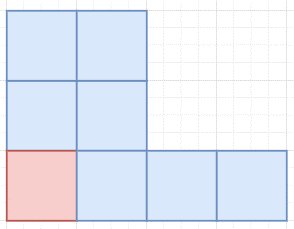
\includegraphics[scale=0.4]{funkydude.png}
        \end{itemize}
    \end{itemize}
    
\end{frame}

%%%%%%%%%%%%%%%%%%%%%%%
\section{Divide and Conquer}

% The Children of $[2, H, 2]$
%%% A
\begin{frame}{fragile}
    \frametitle{The Children of $[2, H, 2]$}
    \framesubtitle{Reordered}
    
    \begin{multicols}{2}
    \begin{itemize}
        \item Group A:
        \begin{itemize}
            \item $[H]$
            \item $[1, 0, 0]$
        \end{itemize}
    \end{itemize}
    \text{$  $} %just for spacing
    
    \begin{itemize}
        \item Group B:
        \begin{itemize}
            \item $[1, H, 2]$
            \item $[0, H, 2]$
            \item $[2, 0, 0]$
        \end{itemize}
    \end{itemize}
    
    \begin{itemize}
        \item Group C:
        \begin{itemize}
            \item $[1, 0, H]$
            \item $[2, 0, 1]$
            \item $[2, 1, 0]$
        \end{itemize}
    \end{itemize}
    
    \begin{itemize}
        \item Group D:
        \begin{itemize}
            \item $[2, H, 2 + K]$
            \item $[2, H, 1]$
            \item $[2, H, 0]$
        \end{itemize}
    \end{itemize}
    \end{multicols}
    
\end{frame}

%%% Group A
\begin{frame}{fragile}
    \frametitle{Group A}
    \framesubtitle{Reduces to 1 x $N$}
    $[H]$\\
    \includegraphics[scale=.4]{[H].png}\\
    $  $\\
    $[1, 0, 0]$\\
    \includegraphics[scale=.4]{[1, 0, 0].png}
\end{frame}

%%%%% [H]
\begin{frame}{fragile}
    \frametitle{$[H]$}
    \framesubtitle{Group A: Reduces to $1$ x $N$}
    
    \begin{multicols}{2}
    $[0, 0, H + 2 + 2]$; \\
    Opponent left only the bottom row\\
    \includegraphics[scale=.4]{images/[H].png}\\
    $[1]$; \\
    Leave only the last piece\\
    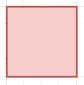
\includegraphics[scale=.4]{images/[1].png}
    \end{multicols}
\end{frame}

%%%%% [1, 0, 0]
\begin{frame}{fragile}
    \frametitle{$[1, 0, 0]$}
    \framesubtitle{Group A: Reduces to $1$ x $N$}
    
    \begin{multicols}{2}
    $[1, H - H, 2 - 2]$; \\
    Opponent broke off all 2’s, all 1’s, and one 3\\
    \includegraphics[scale=.4]{images/[1, 0, 0].png}\\
    $[1]$; \\
    Leave only the last piece\\
    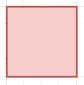
\includegraphics[scale=.4]{images/[1].png}
    \end{multicols}
\end{frame}

% The Children of $[2, H, 2]$
%%% B
\begin{frame}{fragile}
    \frametitle{The Children of $[2, H, 2]$}
    \framesubtitle{Reordered}
    
    \begin{multicols}{2}
    \begin{itemize}
        \item Reduces to $1$ x $N$:
        \begin{itemize}
            \item $[H]$
            \item $[1, 0, 0]$
        \end{itemize}
    \end{itemize}
    \text{$  $} %just for spacing
    
    \begin{itemize}
        \item Group B:
        \begin{itemize}
            \item $[1, H, 2]$
            \item $[0, H, 2]$
            \item $[2, 0, 0]$
        \end{itemize}
    \end{itemize}
    
    \begin{itemize}
        \item Group C:
        \begin{itemize}
            \item $[1, 0, H]$
            \item $[2, 0, 1]$
            \item $[2, 1, 0]$
        \end{itemize}
    \end{itemize}
    
    \begin{itemize}
        \item Group D:
        \begin{itemize}
            \item $[2, H, 2 + K]$
            \item $[2, H, 1]$
            \item $[2, H, 0]$
        \end{itemize}
    \end{itemize}
    \end{multicols}
    
\end{frame}

%%% Group B
\begin{frame}{fragile}
    \frametitle{Group B}
    \framesubtitle{Reduces to 2 x $N$}
    
    \begin{multicols}{2}
    $[1, H, 2]$\\
    \includegraphics[scale=.4]{[1, H, 2].png}\\
    $  $\\
    $[0, H, 2]$\\
    \includegraphics[scale=.4]{[0, H, 2].png}\\
    $  $\\
    $[2, 0, 0]$\\
    \includegraphics[scale=.4]{[2, 0, 0].png}\\
    $  $\\
    $  $\\
    $  $\\
    \end{multicols}
\end{frame}

%%%%% [1, H, 2]
\begin{frame}{fragile}
    \frametitle{$[1, H, 2]$}
    \framesubtitle{Group B: Reduces to $2$ x $N$}
    
    \begin{multicols}{2}
    $[2 - 1, H + 1, 2]$; \\
    Opponent removed one top block\\
    \includegraphics[scale=.4]{images/[1, H, 2].png}\\
    $[1, 1, 0]$; \\
    Break off all but one 2\\
    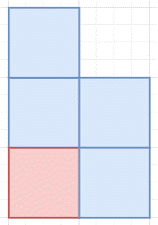
\includegraphics[scale=.4]{images/[1, 1, 0].png}
    \end{multicols}
\end{frame}

%%%%% [0, H, 2]
\begin{frame}{fragile}
    \frametitle{$[0, H, 2]$}
    \framesubtitle{Group B: Reduces to $2$ x $N$}
    
    \begin{multicols}{2}
    $[2 - 2, H + 2, 2 - 2]$; \\
    Opponent broke off both 3's\\
    \includegraphics[scale=.4]{images/[0, H, 2].png}\\
    $[H, 1]$; \\
    Break off the 1 one the end, staircase it\\
    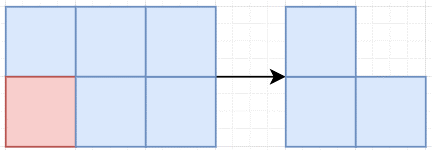
\includegraphics[scale=.4]{images/[H, 1].png}
    \end{multicols}
\end{frame}

%%%%% [2, 0, 0]
\begin{frame}{fragile}
    \frametitle{$[2, 0, 0]$}
    \framesubtitle{Group B: Reduces to $2$ x $N$}
    
    \begin{multicols}{2}
    $[2, H - H, 2 - 2]$; \\
    Opponent broke off all 2’s and all 1’s\\
    \includegraphics[scale=.4]{images/[2, 0, 0].png}\\
    $[1]$; \\
    Break off one 3, Sideways Staircase\\
    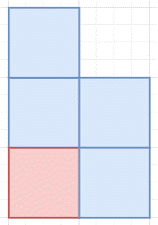
\includegraphics[scale=.4]{images/[1, 1, 0].png}
    \end{multicols}
\end{frame}


% The Children of $[2, H, 2]$
%%% C
\begin{frame}{fragile}
    \frametitle{The Children of $[2, H, 2]$}
    \framesubtitle{Reordered}
    
    \begin{multicols}{2}
    \begin{itemize}
        \item Reduces to $1$ x $N$:
        \begin{itemize}
            \item $[H]$
            \item $[1, 0, 0]$
        \end{itemize}
    \end{itemize}
    \text{$  $} %just for spacing
    
    \begin{itemize}
        \item Reduces to $2$ x $N$:
        \begin{itemize}
            \item $[1, H, 2]$
            \item $[0, H, 2]$
            \item $[2, 0, 0]$
        \end{itemize}
    \end{itemize}
    
    \begin{itemize}
        \item Group C:
        \begin{itemize}
            \item $[1, 0, H]$
            \item $[2, 0, 1]$
            \item $[2, 1, 0]$
        \end{itemize}
    \end{itemize}
    
    \begin{itemize}
        \item Group D:
        \begin{itemize}
            \item $[2, H, 2 + K]$
            \item $[2, H, 1]$
            \item $[2, H, 0]$
        \end{itemize}
    \end{itemize}
    \end{multicols}
    
\end{frame}

%%% Group C
\begin{frame}{fragile}
    \frametitle{Group C}
    \framesubtitle{Reduces to $N$ x $N$}
    
    \begin{multicols}{2}
    $[2, 0, 1]$\\
    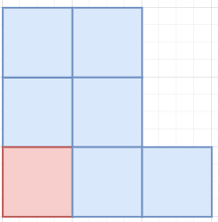
\includegraphics[scale=.4]{[2, 0, 1].png}\\
    $  $\\
    $[2, 1, 0]$\\
    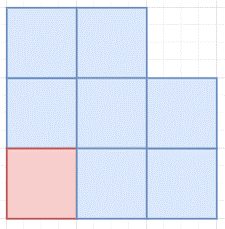
\includegraphics[scale=.4]{[2, 1, 0].png}\\
    $  $\\
    $[1, 0, H]$\\
    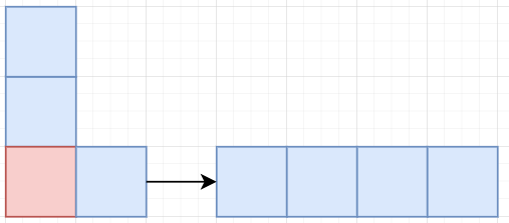
\includegraphics[scale=.4]{[1, 0, H].png}\\
    $  $\\
    $  $\\
    $  $\\
    \end{multicols}
\end{frame}

%%%%% [1, 0, 0]
\begin{frame}{fragile}
    \frametitle{$[1, 0, 0]$}
    \framesubtitle{Group A: Reduces to $1$ x $N$}
    
    \begin{multicols}{2}
    $[1, H - H, 2 - 2]$; Opponent broke off all 2’s, all 1’s, and one 3\\
    \includegraphics[scale=.4]{images/[1, 0, 0].png}\\
    $[1]$; Leave only the last piece\\
    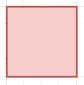
\includegraphics[scale=.4]{images/[1].png}
    \end{multicols}
\end{frame}

%%%%% [1, 0, 0]
\begin{frame}{fragile}
    \frametitle{$[1, 0, 0]$}
    \framesubtitle{Group A: Reduces to $1$ x $N$}
    
    \begin{multicols}{2}
    $[1, H - H, 2 - 2]$; Opponent broke off all 2’s, all 1’s, and one 3\\
    \includegraphics[scale=.4]{images/[1, 0, 0].png}\\
    $[1]$; Leave only the last piece\\
    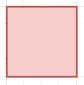
\includegraphics[scale=.4]{images/[1].png}
    \end{multicols}
\end{frame}

%%%%% [1, 0, 0]
\begin{frame}{fragile}
    \frametitle{$[1, 0, 0]$}
    \framesubtitle{Group A: Reduces to $1$ x $N$}
    
    \begin{multicols}{2}
    $[1, H - H, 2 - 2]$; Opponent broke off all 2’s, all 1’s, and one 3\\
    \includegraphics[scale=.4]{images/[1, 0, 0].png}\\
    $[1]$; Leave only the last piece\\
    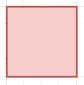
\includegraphics[scale=.4]{images/[1].png}
    \end{multicols}
\end{frame}


% The Children of $[2, H, 2]$
%%% D
\begin{frame}{fragile}
    \frametitle{The Children of $[2, H, 2]$}
    \framesubtitle{Reordered}
    
    \begin{multicols}{2}
    \begin{itemize}
        \item Reduces to $1$ x $N$:
        \begin{itemize}
            \item $[H]$
            \item $[1, 0, 0]$
        \end{itemize}
    \end{itemize}
    \text{$  $} %just for spacing
    
    \begin{itemize}
        \item Reduces to $2$ x $N$:
        \begin{itemize}
            \item $[1, H, 2]$
            \item $[0, H, 2]$
            \item $[2, 0, 0]$
        \end{itemize}
    \end{itemize}
    
    \begin{itemize}
        \item Reduces to $N$ x $N$:
        \begin{itemize}
            \item $[1, 0, H]$
            \item $[2, 0, 1]$
            \item $[2, 1, 0]$
        \end{itemize}
    \end{itemize}
    
    \begin{itemize}
        \item Group D:
        \begin{itemize}
            \item $[2, H, 2 + K]$
            \item $[2, H, 1]$
            \item $[2, H, 0]$
        \end{itemize}
    \end{itemize}
    \end{multicols}
    
\end{frame}

%%% D
\begin{frame}{fragile}
    \frametitle{Group D}
    \framesubtitle{Maintain $[2, H, 2]$}
    
    \begin{multicols}{2}
    $[2, H, 2 + K]$\\
    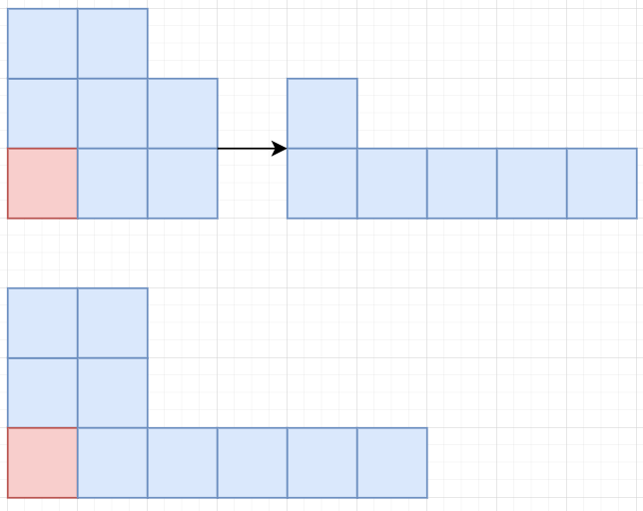
\includegraphics[scale=.4]{[2, H, 2 + K].png}\\
    $  $\\
    $[2, H, 1]$\\
    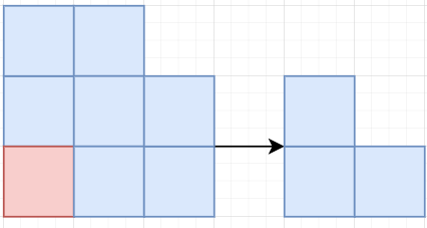
\includegraphics[scale=.4]{[2, H, 1].png}\\
    $  $\\
    $[2, H, 0]$\\
    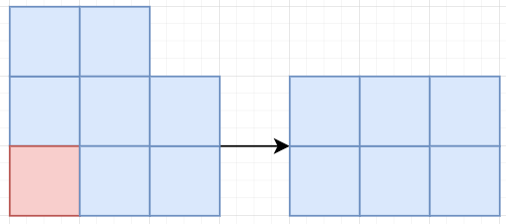
\includegraphics[scale=.4]{[2, H, 0].png}\\
    \end{multicols}
\end{frame}

%%%%% [1, 0, 0]
\begin{frame}{fragile}
    \frametitle{$[1, 0, 0]$}
    \framesubtitle{Group A: Reduces to $1$ x $N$}
    
    \begin{multicols}{2}
    $[1, H - H, 2 - 2]$; Opponent broke off all 2’s, all 1’s, and one 3\\
    \includegraphics[scale=.4]{images/[1, 0, 0].png}\\
    $[1]$; Leave only the last piece\\
    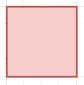
\includegraphics[scale=.4]{images/[1].png}
    \end{multicols}
\end{frame}

%%%%% [1, 0, 0]
\begin{frame}{fragile}
    \frametitle{$[1, 0, 0]$}
    \framesubtitle{Group A: Reduces to $1$ x $N$}
    
    \begin{multicols}{2}
    $[1, H - H, 2 - 2]$; Opponent broke off all 2’s, all 1’s, and one 3\\
    \includegraphics[scale=.4]{images/[1, 0, 0].png}\\
    $[1]$; Leave only the last piece\\
    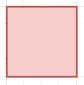
\includegraphics[scale=.4]{images/[1].png}
    \end{multicols}
\end{frame}

%%%%% [1, 0, 0]
\begin{frame}{fragile}
    \frametitle{$[1, 0, 0]$}
    \framesubtitle{Group A: Reduces to $1$ x $N$}
    
    \begin{multicols}{2}
    $[1, H - H, 2 - 2]$; Opponent broke off all 2’s, all 1’s, and one 3\\
    \includegraphics[scale=.4]{images/[1, 0, 0].png}\\
    $[1]$; Leave only the last piece\\
    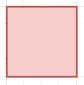
\includegraphics[scale=.4]{images/[1].png}
    \end{multicols}
\end{frame}


% The Children of $[2, H, 2]$
%%% Overview
\begin{frame}{fragile}
    \frametitle{The Children of $[2, H, 2]$}
    \framesubtitle{Reordered}
    
    \begin{multicols}{2}
    \begin{itemize}
        \item Reduces to $1$ x $N$:
        \begin{itemize}
            \item $[H]$
            \item $[1, 0, 0]$
        \end{itemize}
    \end{itemize}
    \text{$  $} %just for spacing
    
    \begin{itemize}
        \item Reduces to $2$ x $N$:
        \begin{itemize}
            \item $[1, H, 2]$
            \item $[0, H, 2]$
            \item $[2, 0, 0]$
        \end{itemize}
    \end{itemize}
    
    \begin{itemize}
        \item Reduces to $N$ x $N$:
        \begin{itemize}
            \item $[1, 0, H]$
            \item $[2, 0, 1]$
            \item $[2, 1, 0]$
        \end{itemize}
    \end{itemize}
    
    \begin{itemize}
        \item Maintain $[2, H, 2]$:
        \begin{itemize}
            \item $[2, H, 2 + K]$
            \item $[2, H, 1]$
            \item $[2, H, 0]$
        \end{itemize}
    \end{itemize}
    \end{multicols}
    
\end{frame}

%%%%%%%%%%%%%%%%%%%%%%
\section{Postamble}
\begin{frame}{fragile}
    \frametitle{Summary and Current Problems}
    
    \begin{itemize}
        \item As far as I can tell, no one else used the truncated forms before
        \item Partial solution and stable boards
    \end{itemize}
    
    $  $\\
    $  $\\
    
    \begin{itemize}
        \item Not very elegant, cases may reduce
        \item Can't reach in one move from $3$ x $N$, but it is stable
    \end{itemize}
\end{frame}

\begin{frame}{Slide Template Credit}
I (Matt Torrence) who has been speaking to you through these slides designed this template myself. Feel free to delete this slide in your presentation.

\s I was inspired by the following stack overflow response and used it as a starting point for this template: \texttt{tex.stackexchange.com/a/146682/188835}

\s Typography used includes 4 typefaces:

\begin{itemize}
\item Charis SIL, for the default serif type
\item \texttt{IBM Plex Mono} for monospace text
\item {\sansstyle Carlito} for the default sans-serif type
\item TeX Gyre Termes Math for all math mode text
\end{itemize}


\end{frame}

\end{document}